%%% chapter of SNO+ detector
%\setlength{\epigraphwidth}{0.5\textwidth}
%\epigraph{In all experimental science the techniques for obtaining measurements are almost as important as the measurements themselves.}{--- \textup{J. D. Bernal}, \textit{The Social Function of Science}}

\section{Overview}\label{sect:overview}

The SNOLAB facility is located at Vale's Creighton mine in Sudbury, Ontario, Canada (coordinates: 46$^\circ$28'19.6"N, 81$^\circ$11'12.4"W), and in particular the SNO+ detector sits deep underground in the mine, beneath a $2092\pm6$ m overburden of rock. This ensures an environment with extremely low cosmic ray backgrounds. At sea level, the average cosmic muon ($\mu$) flux is about $1.44\times 10^7~\mu/\mathrm{m^2/day}$ \cite{muonflux}. Cosmic muons with high energies (mostly $\mathcal{O}$(GeV)) can induce spallation backgrounds, such as fast neutrons and lasting isotopes, which are harmful to experiments of this type because they increase the background count rate, and therefore can obscure ``signal'' events in the sense of widening the confidence intervals on physics findings \cite{beacom2017physics}. The rock overburden above the SNO+ detector reduces the cosmic muon ($\mu$) flux to as low as $0.286\pm0.009~\mu/\mathrm{m^2/day}$, corresponding to 6010 water equivalent meter (m.w.e) \cite{snop_jinst}. Accordingly in each hour, the number of muons passing through the SNO+ detector is $\mathcal{O}(1)$.

The SNO+ detector is a refurbishment of the SNO detector. The SNO+ collaboration makes use of the SNO infrastructure and upgraded it to be a liquid scintillator (as opposed to heavy water) detector. As shown in Fig.~\ref{snopdetector}, the detector is inside a barrel-like rock cavity with a diameter of 22 m at its waist and a height of 34 m. The cavity is filled with 7000 tonnes of ultrapure water (UPW) to provide buoyancy for the detector vessel, and shield radiation backgrounds from the environment, such as the cosmic rays and isotope decays from the rock. 

The detector consists of an acrylic vessel (AV) sphere of 12.01 m diameter and 5.5 cm thickness. The AV contains the detection medium (i.e. target material) and is held in place by a rope net system including hold-up and hold-down Tensylon ropes. This spherical structure is simple in geometry which reduces the complexity of simulation and event reconstruction. Furthermore, this geometry allows for spherical fiducial volume cuts from the center of the AV to reduce the external background count, which makes the SNO+ a ``graded-shield'' type of detector \cite{waterfield2017optical}.
Joined to the top of the AV sphere is an acrylic ``neck'', specifically a cylinder 6.8 m high and 1.46 m in inner diameter. The neck connects the AV sphere to facilities on the deck above. Through the neck, pipes can introduce the detector medium into the AV and recirculate it for purification. Calibration sources for internal scans can also be lowered down into the AV through the neck.

The AV sphere is concentric within, and lies within, a stainless steel geodesic dome having an average radius of 8.4 m, this being the photomultiplier support structure (PSUP). A total of 9394 Hamamatsu R1408 8-inch photomultipliers (PMTs) are mounted on the PSUP, looking inward to the AV. To increase the light collection efficiency of these PMTs and thus to obtain an extensive photocathode coverage of the detector, each of these PMTs was fitted into a 27 cm diameter reflective bucket (called the ``concentrator''), which consists of aluminum-coated reflective petals. The effective photocathode coverage\footnote{Defined as the fraction of a large sample of photons, emitted isotropically at the origin, that enter a PMT.} of the detector is about 54\% \cite{whitepaper}. In addition to the inward-looking PMTs, a further 90 PMTs look outward, serving as muon vetos. Four Hamamatsu R5912 High Quantum Efficiency (HQE) PMTs were also installed, in order to test their performance for a potential further phase of the SNO+ experiment \cite{stringer2019sensitivity}.

\begin{figure}[htbp]
	\centering
	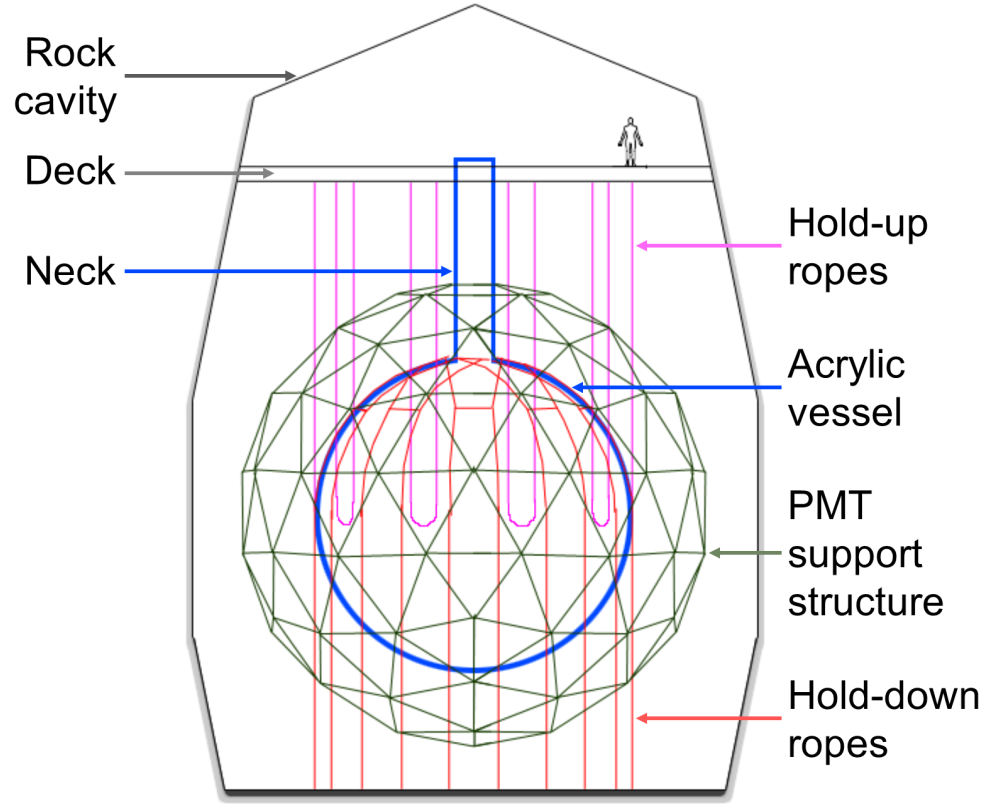
\includegraphics[width=10cm]{SNOPdetector.png}
	\caption[The SNO+ detector labeled with main structures.]{The SNO+ detector labeled with main structures, modified from Ref.~\cite{jones2011background}.}
	\label{snopdetector}
\end{figure}

\section{SNO+ Physics Phases}\label{sect:physicsPhase}

The SNO+ experiment is designed for multi-purpose measurements of neutrino physics, and the detector has been in operation since December 2016. There are three physics phases of the experiment, each phase having a different detection medium inside the AV: the water phase, the scintillator phase, and the tellurium phase \cite{whitepaper}. 

\subsection{Water Phase} \label{sect:waterPhase}

In this initial phase, about 905 tonnes of ultrapure water was contained in the AV. The detector collected water physics data from May 2017 to July 2019.

During the data-taking, different types of calibration runs were performed. The detector timing and energy response, systematics, and backgrounds were studied. Numerous analyses, e.g. of invisible nucleon decay, solar neutrinos, and reactor antineutrinos, are ongoing, and related findings have been published \cite{anderson2019search,anderson2019measurement,anderson2020measurement,anderson2021optical}. The external backgrounds\footnote{That is, event types and rates due to radioactive sources other than those producing the signals of interest, in particular decays occurring outside the detector in the rock mass and the water cavity, as well as those due to low level radioactive contamination of the acrylic AV wall, and so forth.} have also measured, and these will be unchanged over the subsequent two phases.

In this first phase, i.e. the water phase, the main physics goal is to search for invisible nucleon decay, whose occurrence is predicted by Grand Unified Theory (GUT) and would violate the baryon number conservation rule of the SM. In the putative ``invisible'' decay mode, a proton or a bound neutron decays without releasing charged particles, in contrast to the (again, putative) ``visible'' decay channels\footnote{Whether visible or invisible, these hypothesized events lie outside the SM, because they violate baryon number conservation.} of $p\to e^+ \pi^0$ and $p\to\nu K^+$, for which the Super-K experiment searched and set limits. In the SNO+ water detector, a $^{16}$O nucleus may decay into a $^{15}$O$^*$ (bound neutron invisible decay) or a $ ^{15}$N$^*$ (proton invisible decay) excited state. The $^{15}$O$^*$ has 44\% chance to de-excite to produce a 6.18-MeV $\gamma$ ray and a 2\% chance to produce 7.03-MeV $\gamma$; while $^{15}$N$^*$ has a 41\% probability to release a 6.32 MeV $\gamma$ and a (2\%, 2\%,3\%) probability to release (respectively) a (7.01, 7.03, 9.93) MeV $\gamma$. The SNO+ experiment has searched for these $\gamma$ signals and published world-leading limits of $\mathcal{O}(10^{29})$ years for both the proton and the neutron invisible decay lifetime at 90\% Bayesian credibility level \cite{anderson2019search}. 

The $^8$B solar neutrinos were measured with a 69.2 kilo-tonnes$\cdot$day dataset. By analyzing solar neutrino elastic scattering events based on the dataset (Chapter 6 will discuss the method in detail), the number of the solar neutrino events were counted in different energy regions. In the first publication \cite{anderson2019measurement}, by fitting to the {\em non-oscillating} solar neutrino model the data provided an estimate $2.53^{+0.31}_{-0.28}(stat.)^{+0.13}_{-0.10}(syst.)\times 10^6$ cm$^{-2}$s$^{-1}$ for the number flux of $^8$B solar neutrinos having energies larger than 5 MeV. In the energy region larger than 6 MeV, the dataset has a background rate of $0.25^{+0.09}_{-0.07}$ events/kilo-tonne$\cdot$day, which is extremely pure with solar neutrinos. Currently, this background rate is the lowest among the class of water Cherenkov detectors \cite{anderson2019measurement}. 

Reactor antineutrinos can be captured by the SNO+ detector and measured. 40\% of these antineutrinos are from one nearby reactor complex in Canada at a distance of 240 km; 20\% are from two Canadian complexes at around 350 km; the remainder arrive from the USA and elsewhere with longer baselines \cite{whitepaper}. Though the detectable antineutrino event rate in pure water is much lower than in the scintillator, during the water phase, SNO+ still has the potential to detect reactor antineutrinos due to the low background dataset and relatively high detection efficiency. An Americium-Beryllium (AmBe) calibration source was deployed during the water phase to evaluate the sensitivity for detecting reactor antineutrinos. This source provides neutrons along with 4.4 MeV $\gamma$ particles. The neutrons are captured by hydrogen, upon each which occurrence a 2.2 MeV photon is released. An analysis of delayed coincidence between 4.4 MeV and 2.2 MeV photons can help tag neutrons, which is crucial for tagging the reactor antineutrinos since they are measured by the inverse $\beta$-decay process, which also produces neutrons with a similar energy scale. In the first publication for the SNO+ water phase, a neutron detection efficiency of 50\% was obtained when the AmBe source was deployed at the center of the detector; the neutron-hydrogen capture time constant $\tau$ was measured to be $202.35_{-0.76}^{+0.87}~\mu s$, and from $\tau$, a thermal capture cross-section was calculated to be $336.3^{+1.2}_{-1.5}$ milli-barn (mb) \cite{anderson2020measurement}.

\subsection{Scintillator Phase} \label{sect:scintPhase}

In this phase, the AV will be filled with 780 tonnes of liquid scintillator, which is a mixture of linear alkylbenzene (LAB) serving as solvent and 2,5-diphenyloxazole (PPO) serving as fluor, with a concentration of 2 gram PPO per liter LAB (2 g/L in short). This LAB-based organic liquid scintillator is denoted as the ``unloaded'' liquid scintillator (more details in Sect.~\ref{sect:LS_SNO+}).

As mentioned in Sect.~\ref{sect:futureSolar}, the main physics goal of the scintillator phase is to measure low energy solar neutrinos: the CNO, pep, and low energy $^8$B neutrinos. Three kinds of antineutrinos will also be measured: reactor antineutrinos (mentioned before), geoneutrinos (from natural radioactivity in the Earth); and supernova neutrinos. SNO+ is intended to join the SuperNova Early Warning System (SNEWS), which is an international network of experiments with the ability to provide an early warning of a galactic supernova \cite{snop_jinst}.

\subsection{Partial-fill Phase} \label{sect:partialPhase}

Between the water phase and the scintillator phase, the liquid scintillator occupied a gradually increasing proportion of the AV volume, as it progressively replaced the water. The liquid scintillator, being insoluble in and having a lower density than water, formed a layer standing above the water. Over certain intervals during the fill, the level of the scintillator/water interface the mixing ratio of PPO in the LAB were stable, and these stable stages were sustained for a few weeks in order to take data under steady conditions. These transition stages were denoted as ``partial-fill phase''. Analyses on the partial-fill phase data are mainly aimed to demonstrate in a trial setting the techniques to be used with liquid scintillator before arriving at that (scintillator) phase, and to test the physical properties of the liquid scintillator, such as the light yield, the background levels, etc. Due to the Covid19 pandemic, the duration of the partial-fill phase proved to be longer than had been planned, accidentally providing more data for some of the intended physics studies, such as measuring solar neutrinos.

\subsection{Tellurium Phase} \label{sect:tePhase}

In the final, ``Te-loaded scintillator'' phase, 1.3 kilo-tonnes of $^{130}$Te will be loaded into the scintillator to achieve a planned mixing ratio of 0.5\% natural Tellurium (Te) by mass (more details in Sect.~\ref{sect:TeLS_SNO+}). Higher loading concentrations would be possible for a further loading plan \cite{Paton:2019kgy}. The main purpose of this phase is to search for the $0\nu\beta\beta$ signals in $^{130}$Te.

\section{Detection Media} \label{sect:detectionMedia}

In the SNO+ detector, charged particles interact with the detection medium and create Cherenkov light and scintillation light. 

\subsection{Cherenkov Radiation}\label{sect:cherenkov}

For any charged particle traveling in a transparent medium at an ultra-relativistic speed (a speed greater than the local phase speed of light in the medium), a type of electromagnetic radiation, called Cherenkov radiation, can be emitted from the coherent response of the medium under the action of the field of the moving particle \cite{jackson2007classical,landau2013electrodynamics}.

Suppose a charged particle moves in a transparent, isotropic, and non-magnetic medium and creates an electromagnetic wave. The electromagnetic wave propagates with a wavenumber $k=\omega/v_p \equiv n\omega/c$, where $c$ is the speed of light in vacuum, $\omega$ is the frequency, $n=n(\omega)$ is the real-valued refractive index and $v_p=c/n(\omega)$ is the phase velocity in the medium. If the particle travels uniformly along the $x$-axis with speed $v>v_p$, Cherenkov radiation of frequency $\omega$ is emitted \cite{landau2013electrodynamics}. The ``Cherenkov angle'', $\theta_\mathrm{Ch}$, is the angle between the direction of motion of the particle and the direction of Cherenkov emission, and it is given by 
\begin{equation}
\cos\theta_\mathrm{Ch}(\omega) = \frac{c}{n(\omega)v} \; .
\end{equation}
The radiation is distributed over the surface of a cone with the half-opening angle $\theta_\mathrm{Ch}$. 

Now consider the the case of an electron traveling in a water detector: what threshold speed and energy must the electron possess, in order to promote Cherenkov radiation? Taking $n_{water}\simeq 1.33$ \cite{pdg2020}, i.e. neglecting the dependence of $n$ on $\omega$, we obtain a threshold speed $v^{\mathrm{min}} = v_p \simeq 2.254\times10^8~m/s$. This corresponds to a kinetic energy:
\begin{equation*}
E_k=(\gamma-1)mc^2=0.264~\mathrm{MeV},
\end{equation*}
where $\gamma=1/\sqrt{1-v_p^2/c^2}$. This is the lowest kinetic energy to create Cherenkov radiation in water, and is referred to as the Cherenkov threshold ($E_{\mathrm{thresh}}$). The corresponding Cherenkov angle is $\theta_\mathrm{Ch}\simeq 41.25^\circ$. For the LAB-PPO (scintillator) medium, $n\simeq 1.50$ \cite{tseung2011ellipsometric}, giving threshold electron (kinetic) energy $E_{\mathrm{thresh}}\simeq 0.175$ MeV and $\theta_\mathrm{Ch}\simeq 48.19^\circ$.
For a particle with a charge of $ze$, the number of photons produced by Cherenkov radiation per unit path length and per unit frequency of the photons is given by \cite{leo2012techniques}
\begin{equation}
\frac{d^2N}{d\omega dx}=\frac{\alpha (ze)^2}{c}\sin^2\theta_\mathrm{Ch}=\frac{\alpha (ze)^2}{c} \; \left(1-\frac{1}{\beta^2 n^2(\omega)} \right) \, ,
\end{equation}
where $\alpha$ is the fine structure constant and $\beta=v/c$. Substituting $\omega= (2\pi c)/\lambda$ and integrating over a wavelength band $\lambda_1 \le \lambda \le \lambda_2$, the number of photons produced per unit of distance along the $x$-axis (i.e. particle path) within that waveband is \cite{leo2012techniques}:
\begin{equation}
\frac{dN}{dx}=2\pi \alpha (ze)^2\sin^2\theta_\mathrm{Ch}\int_{\lambda_1}^{\lambda_2}\frac{d\lambda}{\lambda^2} \; .
\end{equation}
For optical photons with wavelengths ranging from $350$ to $550 \; \mathrm{nm}$ (a typical PMT sensitivity range), the above formula evaluates to \cite{leo2012techniques}:
\begin{equation}
\frac{dN}{dx}=476(ze)^2\sin^2\theta_\mathrm{Ch} \; \mathrm{photons/cm}.
\end{equation}
For Cherenkov radiation caused by electron motion in a water detector, $dN/dx \simeq 207 \; \mathrm{photons/cm}$; while in the LAB-PPO case, $dN/dx \simeq 264 \; \mathrm{photons/cm}$. In more detailed accounting, PMT coverage and detection efficiency need to be admitted into the derivation.

\subsection{Scintillation Light from Organic Scintillator}\label{sect:scintillator}

When charged particles travel through an organic scintillator the importance of Cherenkov radiation is much reduced, relative to ``scintillation photons'', which are produced as follows. 

An organic liquid scintillator is composed of aromatic hydrocarbon compounds with benzene-ring structures, and ionizing radiation may excite the free valence electrons of the molecules into the $\pi$-molecular orbitals with the benzene rings. These highly delocalized electrons can occupy a series of energy levels, as shown on a Jablonski diagram (Fig.~\ref{jablonski}) which represents these $\pi$-electronic energy levels \cite{knoll2010radiation,leo2012techniques}. 
\begin{figure}[!htb]
	\centering
	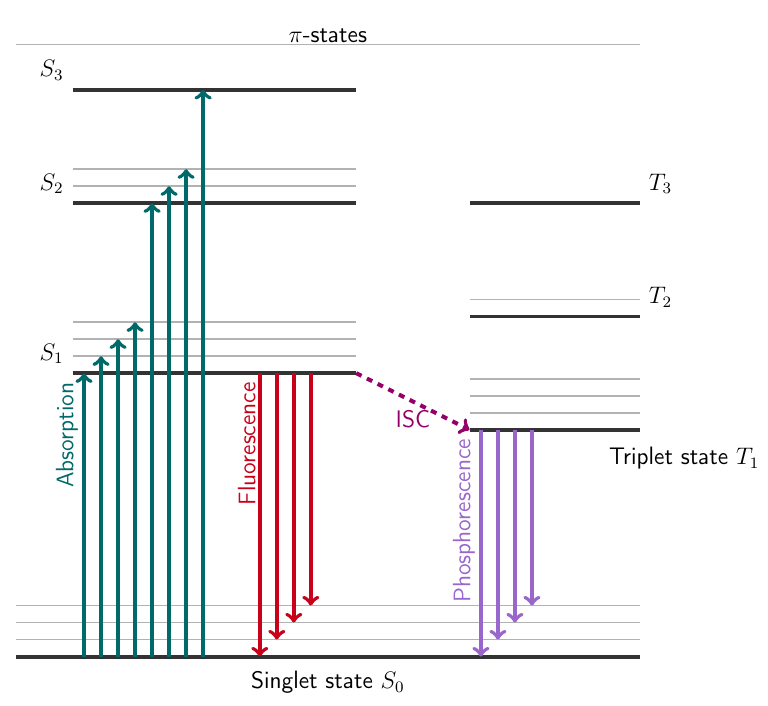
\includegraphics[width=10cm]{jablonski.png}
	\caption[A Jablonski diagram for the organic scintillator.]{A Jablonski diagram for the organic scintillator, modified from Refs.~ \cite{birks1965theory, knoll2010radiation}.}
	\label{jablonski}
\end{figure}
%, invented by Polish physicist Aleksander Jab\l o\'{n}ski, 
In the diagram, $S_{0,1,2,3,...}$ are the energy levels of the spin-0 singlet states, where $S_0$ is the ground state and $S^*=S_{1,2,3,...}$ are the excited singlet states. Above the ground state $S_0$, there are also a set of spin-1 triplet states $T_{1,2,3,...}$, where $T_1$ is the lowest triplet state. These electron energy levels are labeled with thick black lines. The energy spacings between these levels are $\mathcal{O}$(eV). In each level, there are also fine structure levels that correspond to excited vibration modes of the molecule (labeled with gray lines and typically labelled as $S_{10}, S_{11}, ..., S_{20}, S_{21}, ...$). The energy spacings between these fine levels are $\mathcal{O}(0.15)$ eV \cite{leo2012techniques, knoll2010radiation}.

The ionizing radiation transfers energy to the molecules and excites the electron levels as well as the vibrational levels, labeled as the absorption lines (in green). The decays between the excited singlet states (not to the ground state) are almost immediate ($\leq 10~$ps), and occur without emission of photons, a process called internal degradation. The decays from the excited singlet state $S_1$ (as well as from the vibrational states $S_{10},S_{11},S_{12},...$) to the ground state (or to the vibrational excitations of it, i.e. to $S_{01}, S_{02}, ...$) happen promptly ($\mathcal{O}$(ns)) and emit light (these transitions are shown as red lines): this is the {\em fluorescence} process, which contributes the prompt component of the emitted scintillation light. The probability that an $S_1$ state decays to one of the vibrational states $S_1 \to S_{01},S_{02},...$ exceeds the probability of a decay to the ground state $S_0$. Since the (photon) energy absorbed to enable the $S_0 \to S_1$ transition is larger than the emitted photon energy of the decays $S_1 \to S_{01}, S_{02},...$, organic scintillators exhibit very little self-absorption of (their own) fluorescence light, and so are effectively transparent to their own radiation. The effect of Stokes shift, which refers to the overlap between the optical absorption and emission spectra, is small \cite{leo2012techniques,knoll2010radiation}. 

Transitions between the singlet and triplet states are highly forbidden, as electron spin-flip is involved \cite{von2015measurement,sorensen2016temperature}, leaving the question: how are the triplet states populated? There does exist a relatively rare process called intersystem crossing (ISC), which converts excited singlet states into triplet states. But most often (with 75\% probability) triplet states are be produced by ionization-recombination \cite{von2015measurement,dunger2018topological}.
%\color{red}Do you need to add a sentence or two expanding on this mechanism Jie?\color{black}.

As to the de-excitation of triplet states, there is again a similar processes of internal degradation taking states $T_{2,3, ...}$ to state $T_1$. $T_1$ however is a relatively stable state, as indicated by the fact that the mean lifetime of a molecule in the triplet state is $\mathcal{O}(10^{-4}~-~10)$ s \cite{mcquarrie1997physical}. This stability owes to the fact that the direct transition $T_1\to S_0$ is highly forbidden. However, the $T_1$ state can undergo an indirect decay process by interacting with another excited $T_1$ molecule to form an excited singlet state:
\begin{equation}
T_1+T_1\to S^*+S_0 \text{ + phonons}.
\end{equation}
The $S^*$ state will then de-excite, emitting delayed scintillation light. This process is called ``delayed fluorescence'' or (perhaps more commonly) ``phosphorescence'' \cite{leo2012techniques}, and contributes the delayed component of scintillation light.

For a typical scintillator detector, the time scale of detector response is $\mathcal{O}(1-100)$~ns. In this time region, the emission of the scintillation light contains the primary fluorescence from the de-excitation of the singlet states (prompt component) and the delayed fluorescence from the de-excitation of the indirect triplet states (delayed component) \cite{dunger2018topological}. The time profile of the scintillation light is a mixture of prompt and delayed components. 

Different charged particles can cause different ionization densities when they deposit energy to the scintillator molecules. The ionization density affects the relative populations of the excited singlet and triplet states. Compared to an electron, an $\alpha$-particle causes a high ionization density, producing a higher ratio of triplet states to singlet states. Therefore, the time profile for the $\alpha$-particle has more delayed light (or longer tails) than that of the electron. This enables the organic scintillator detector to distinguish an $\alpha$ particle from an electron or other lighter charged particle \cite{dunger2018topological, collaboration2020development}.
An empirical formula, Birk's law \cite{birks1951scintillations, birks1965theory}, describes the photon yield per unit distance produced by the incident particle:
\begin{equation}
\frac{dY}{dx}=A \, \frac{dE/dx}{1+k_B \, dE/dx} \, ,
\end{equation}
where $A$ is a normalization constant and $k_B$ is the Birks' constant of the scintillator, which in practice is obtained by fitting the formula to measured data.

\subsection{Liquid Scintillator for SNO+}\label{sect:LSproperty}

Organic scintillators can offer a high light yield at wavelengths in the sensitive wavelength band of the detector's PMTs and (as seen above) have characteristics that are useful in the context of particle identification. In addition, since organic liquids are non-polar media, the solubility of ionic impurities within them is low. This leads to lower contamination levels of uranium (U), thorium (Th), and potassium (K) in organic liquid scintillators. Among the organic scintillators, aromatic organic liquid scintillators have high electron densities and thus provide sufficiently numerous targets for particle interactions \cite{PerkinElmer}. Due to these advantages, aromatic organic liquid scintillators have been extensively developed as detection media for large particle detectors, especially for neutrino experiments, such as KamLAND, Borexino, Day Bay, and JUNO \cite{collaboration2020development}.

The SNO+ project has developed such a liquid scintillators, compatible with the detector components and notably with the acrylic material of the AV sphere. Two kinds of SNO+ liquid scintillators are discussed in the following sub-sections: the unloaded liquid scintillator for the scintillator phase and the Tellurium-loaded liquid scintillator (TeLS) for the tellurium phase.

\subsection{Water-based Wavelength Shifter (Proposal)}\label{sect:wbWLS}

X. Dai et al. \cite{dai2008wavelength} proposed adding wavelength shifter (WLS) into a water Cherenkov detector like SNO. Relative to a water Cherenkov detector, a detector using a water-based wavelength shifter (wbWLS) has a higher light yield (about threefold higher than SNO \cite{dai2008wavelength}) and thus has a lower energy threshold for particle detection, i.e. low energy events. At the same time, such a detector retains the directionality characteristic of the Cherenkov signal, in contrast to the case of a liquid scintillator detector. For studying directional signals such as solar neutrinos, this directionality is helpful for suppressing the background events. This technology is being studied by future neutrino experiments, such as the Advanced Scintillation Detector Concept (ASDC) \cite{alonso2014advanced}, WATCHMAN experiment \cite{askins2015physics} and Jinping experiment \cite{beacom2017physics}.

The U.~Alberta group made a proposal of adding wavelength shifter (WLS) into the SNO+ detector in the middle of the water phase. The specific wavelength shifter we considered is PPO, which is a well-studied ingredient of the liquid scintillator used in the SNO+ scintillator phase and Te-loaded phase. It can be dissolved into water by mixing with a suitable water-surfactant. Although this proposal was not adopted due to the experiment schedule, it is still worthwhile for a conceptual study of a SNO+-like detector that uses water-based wavelength shifter (wbWLS) as the detection medium. In Sect.~\ref{sect:WLSfitter}, Chapter 4, an event reconstruction algorithm based on the use of wbWLS is discussed. This algorithm that relative to an ordinary water-Cherenkov detector, the energy threshold can be lowered and the resolution of the reconstructed event position improved, while still retaining the directionality response (i.e. permitting to reconstruct the direction of the incoming particle's path from the Cherenkov light). This feature will help for measuring low energy solar neutrinos.

\subsection{Unloaded Liquid Scintillator}\label{sect:LS_SNO+}

SNO+ adopted a liquid scintillator cocktail containing two primary components: LAB as solvent and PPO as solute. The LAB will be doped with PPO to a concentration of 2 g/L. This mixture of the LAB and 2 g/L PPO is denoted as the unloaded liquid scintillator in the text. Fig.~\ref{labppo-molecule} shows the chemical structural formulae of LAB and PPO \cite{collaboration2020development}.
\begin{figure}[!htb]
	\centering
	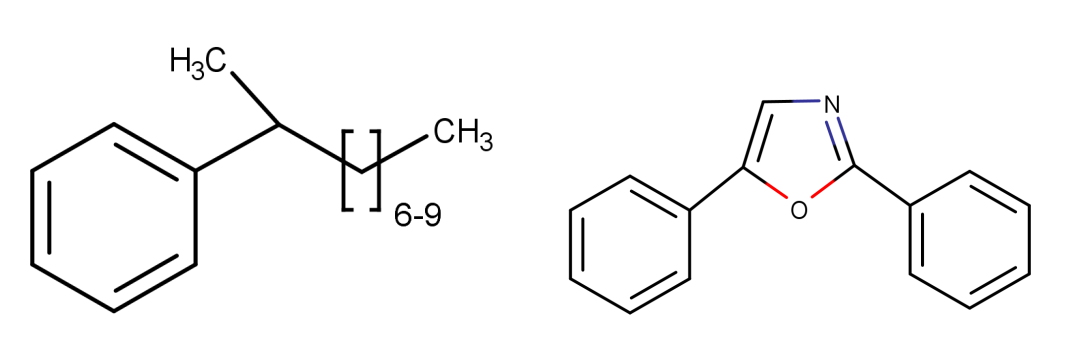
\includegraphics[width=8cm]{lab-ppo-molecule.png}
	\caption[Structural formulae of LAB and PPO.]{Structural formulae of LAB (left) and PPO (right).}
	\label{labppo-molecule}
\end{figure}

LAB is a family of alkylated aromatic organic compounds with a phenyl group attached to a long carbon chain varying from 9 to 14 carbons \cite{wiki_LAB, collaboration2020development}. It has been used as a biodegradable surfactant to detergent since the 1960s and is known to be relatively non-toxic, and carry very low risk for the environment and for human health \cite{wiki_LAB}. Due to the long carbon chain, LAB is an effective energy absorber to transfer the energy deposited by a passing charged particle into light. It also has a long attenuation length of ($72\pm 14$) m at 546 nm and thus has good optical transparency \cite{snop_jinst}. Fig.~\ref{absLength} shows the absorption lengths of SNO+ optical components, comparing the LAB, PPO to the water.
\begin{figure}[!htb]
	\centering
	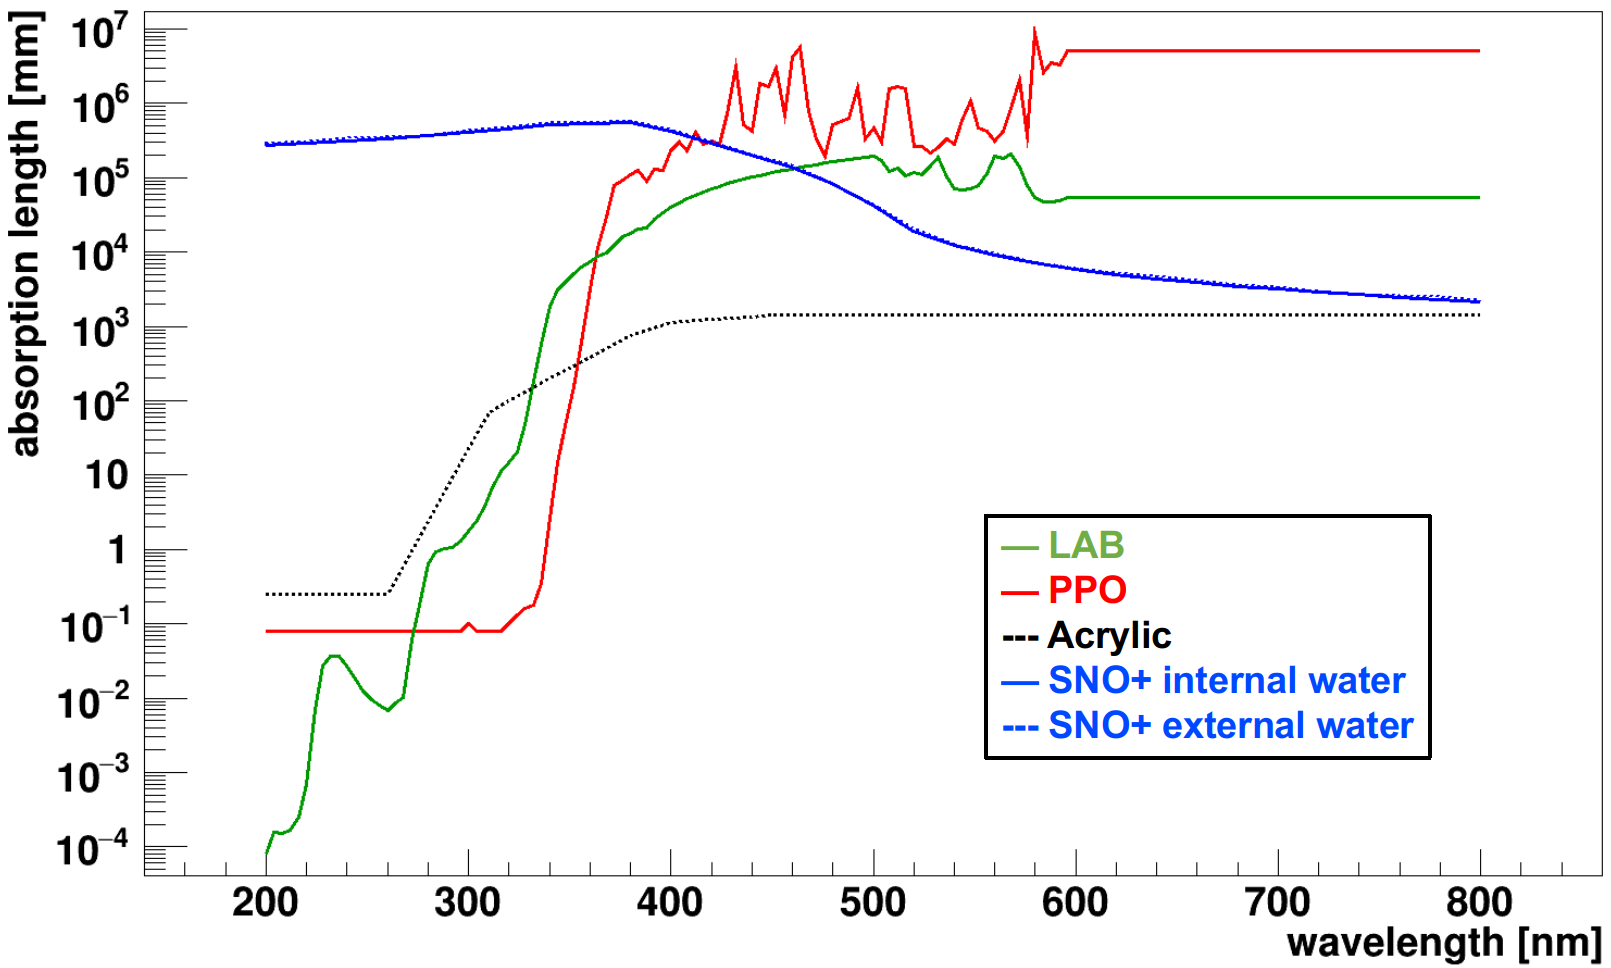
\includegraphics[width=12cm]{absLength.png}
	\caption[Spectral absorption length for SNO+ optical components.]{Spectral absorption length for individual SNO+ optical components. The internal (solid blue line) and external water (dashed blue line) absorption curves are based on the measurements of the laserball scans in July 2018 during the SNO+ water phase. The horizontal lines are a conservative extrapolation to wavelengths at which measurements are lacking.}
	\label{absLength}
\end{figure}

As discussed above, PPO is dissolved into the LAB so it may function as a wavelength shifting fluor \cite{wunderly1990new}. Energy is transferred from LAB to PPO via non-radiative F{\"o}rster resonant energy transfer, bypassing or short-circuiting the other de-excitation modes of the LAB. The outcome is that radiant de-excitation of the PPO (fluor) occurs at scintillation photon wavelengths in a range of 300-550 nm, better suited to the PMT's sensitivity range. In addition, the PPO-doped cocktail results in reduced self-absorption of scintillation light (better optical transparency). 

The 2 g/L PPO concentration in LAB is considered optimal for the purposes of SNO+ \cite{whitepaper}. The absolute light yield of the LAB+ 2g/L PPO mixture has been well-measured from large particle physics experiments \cite{xing2015preliminary,agostini2018comprehensive}, as well as bench-top measurements \cite{xing2015preliminary,kaptanoglu2019cherenkov, novikov}. The value determined by SNO+ is $11900\pm 60$ photons/MeV, and this is expected to be increased by over 15\% after an extensive purification process \cite{snop_jinst,grullon2014light}. At the 2 g/L PPO concentration, the emission decay time is about 5 ns, which is good enough for event vertex reconstruction, and this fast timing ensures distinct timing spectra for $\alpha$ and $\beta$ events, which is crucial for $\alpha/\beta$ discrimination and reducing the backgrounds \cite{snop_jinst}. 

During the SNO+ partial-fill phase, intervals of detector operation are available with steady values of PPO mixing ratio at 0.25 g/L, 0.5 g/L and 1 g/L concentrations. When the PPO concentration increases, the PPO transfer efficiency will increase, which can increase the light yield of the liquid scintillator, and also cause a faster scintillation timing response. However it was found that there is little to be gained by allowing the PPO concentration to exceed 2 g/L, due to an increase in self-absorption (such that light yield reaches a plateau) and a slightly accelerated timing response (see Sect.~\ref{sect:differentPPOconcen}, Chapter 4 for more details) \cite{snop_jinst,collaboration2020development}. In Sect.~\ref{sect:ppoConcentration}, Chapter 4, I show the effects of the PPO concentration on event position reconstruction. As PPO concentration increases from 0.25 g/L to 2 g/L, the resolution in reconstructed event position (for 3-MeV electron events) is refined by about 9 cm. However as PPO concentration increases from 2 g/L to 6 g/L there is almost no change in light yield, demonstrating that 2 g/L PPO concentration is for all intents and purposes optimal.

Scintillator light emission time profiles were obtained from bench-top measurements. An empirical model for the response, consisting of $n$ ($n$=3 or 4) exponential decays with a common rise time, is used to describe (i.e. fit) the time profiles \cite{biller2020slow}, viz.
\begin{equation}
\sum^{n}_{i=1}A_i\cdot\frac{e^{-\frac{t}{\tau_i}}-e^{-\frac{t}{\tau_{\mathrm{r}}}}}{\tau_i-\tau_{\mathrm{r}}},
\end{equation}
where the rise time ($t_{\mathrm{r}}$), timing parameters $t_i$, and amplitude $a_i$ of any given liquid scintillator must be determined by measurements. Fig.~\ref{fig:allTiming} plots the time profiles based on the measured parameters from the collaboration \cite{chicagoTiming,tanner0p5,tannerTeDDA,joshW1}. It shows the time profiles of four different liquid scintillator cocktails planned for SNO+, including the LAB + 0.5g/L PPO for the partial-fill phase, which will be discussed in Chapter 4; the LAB + 2g/L PPO for the scintillator phase; the LAB + 2g/L PPO + 0.5\% molar concentrations DDA, which will be a transient state before loading of the Te; and the LAB + 2g/L PPO + 0.5\% molar concentrations Te+0.5\% molar DDA for the tellurium phase. For each liquid scintillator, the timing responses to $\alpha$- (dashed lines) and $\beta^-$- (solid lines) particles are shown. This figure shows that with 2 g/L PPO there is obvious difference between the $\alpha$ and $\beta^-$ timing, while for the 0.5 g/L PPO, such difference is not obvious. However, some recent SNO+ \emph{in-situ} data analyses (relating to the ``Berkeley AlphaBeta Classifiers'') based on the partial-fill data still show some ability to distinguish $\alpha$- and $\beta^-$- particles by their time profiles \cite{maxSmileyBerkeleyAlphaBeta}. 

\begin{figure}[!htb]
	\centering
	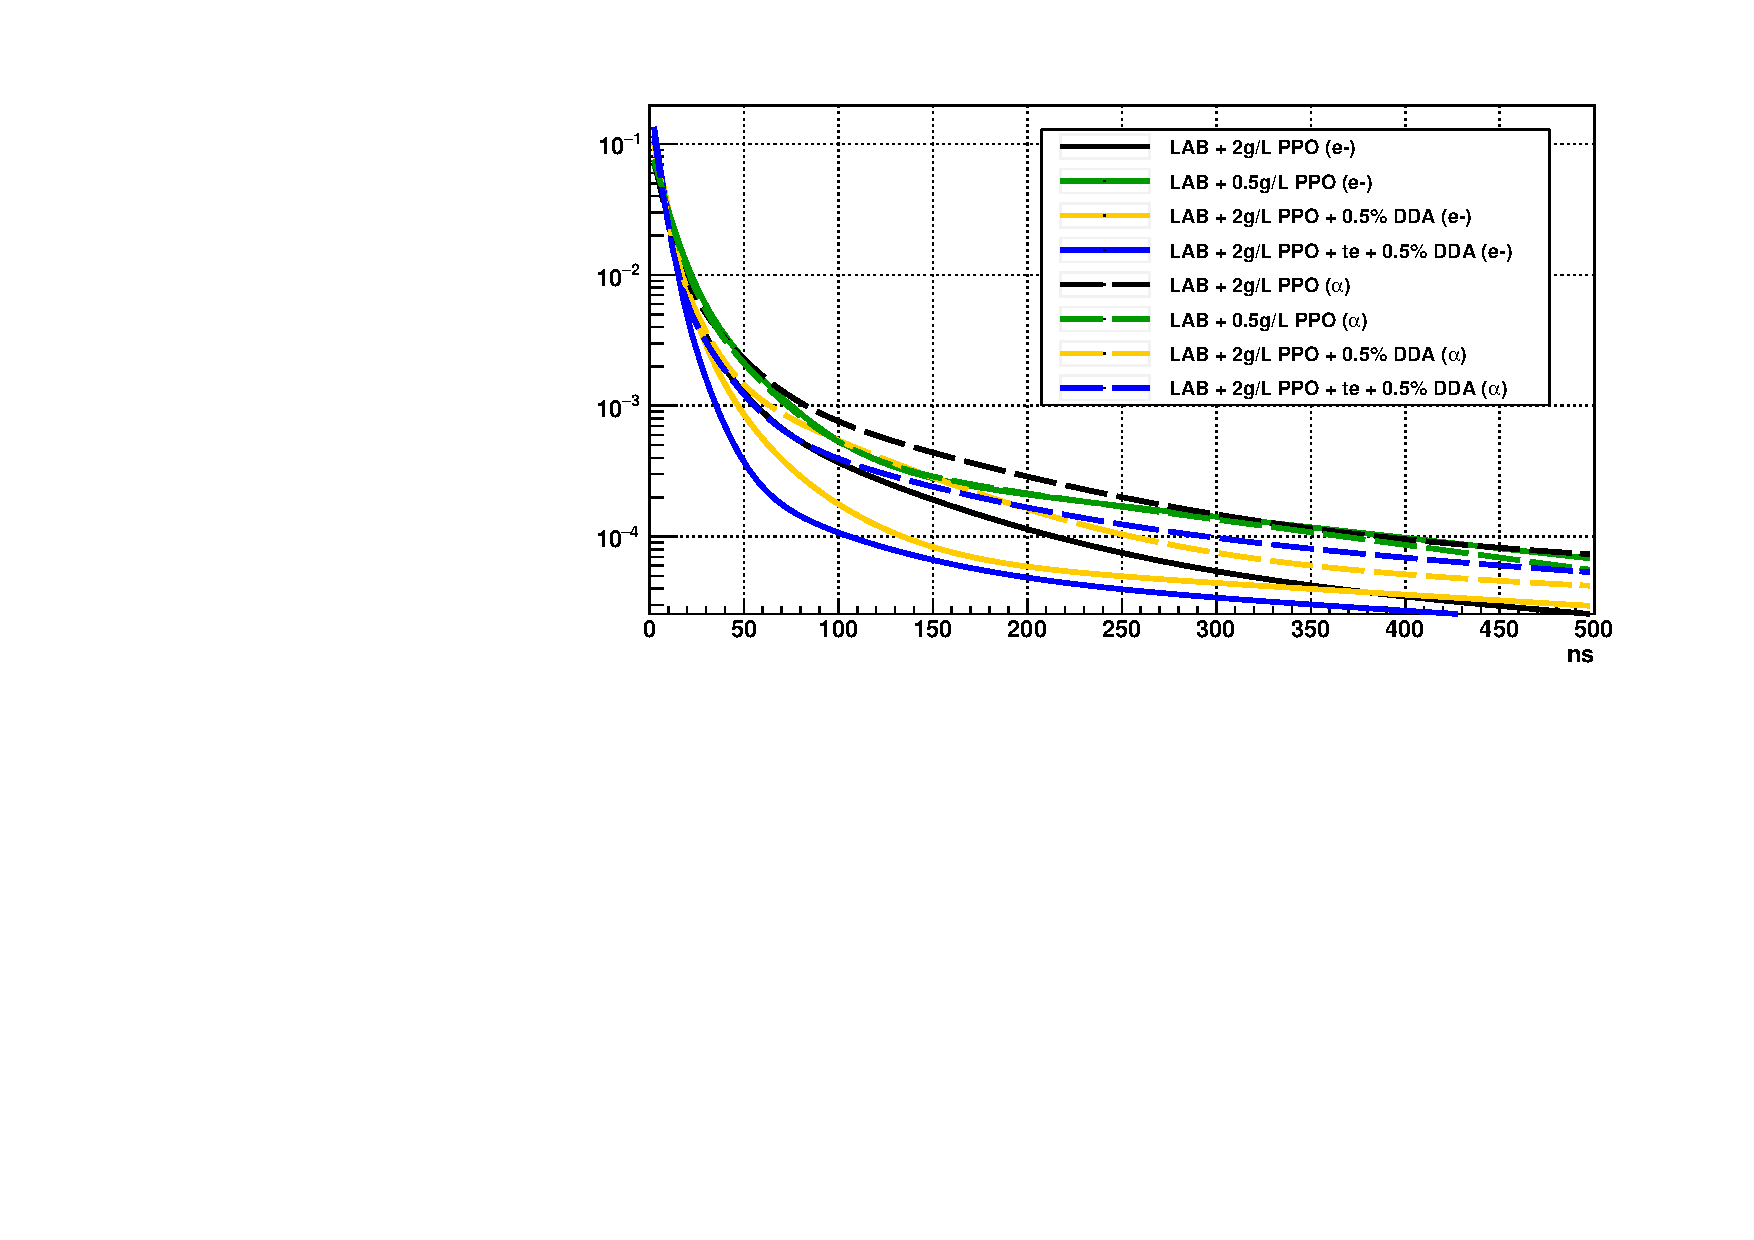
\includegraphics[width=10cm]{plotAllTiming.pdf}
	\caption{Time profiles for liquid scintillators in different SNO+ phases.}
	\label{fig:allTiming}
\end{figure}

The LAB and the PPO used by SNO+ are ultrapure, with very low levels of natural radioactive contaminants such as U, Th and K. The target background levels for the SNO+ LAB are expected to be $\mathcal O(10^{-17})$ gram of $^{238}$U per gram LAB (g$^{238}$U/gLAB), which taking account of the detector volume equates to $\mathcal{O}\left[10^3\right]$ events per year. The $^{232}$Th and $^{40}$K contamination levels are equally low, i.e. $\mathcal O(10^{-17})$ g/gLAB, but due to their longer half-lives their event rates in the detector are $\mathcal{O}\left[10^2\right]$ events per year \cite{snop_jinst,markchen_bkg}. A liquid scintillator purification plant has been implemented to maintain the optical clarity and radiopurity of the scintillator \cite{snop_jinst}.

\subsection{Tellurium-loaded Liquid Scintillator}\label{sect:TeLS_SNO+}

To load the $^{130}$Te into the liquid scintillator, an organo-metallic compound, called ``Tellurium Butanediol (TeBD)'', is formed by condensation (or ``diolization'') reactions between telluric acid (TeA) and 1,2-butanediol (BD) \cite{Paton:2019kgy}. A tertiary amine ``DDA'' (for N, N-Dimethyldodecylamine) is added during the reaction to stabilize TeBD compounds and avoid any phase separation \cite{teLoadingPaper}. Fig.~\ref{fig:paton_te} shows initial stages of the process. This compound is then loaded into the liquid scintillator.
\begin{figure}[!htb]
	\centering
	
\includegraphics[height = 3cm]{TeBD_process.png}
	\caption{Initial stages of the TeBD compound formation, modified from Ref.~\cite{Paton:2019kgy}.}
	\label{fig:paton_te}
\end{figure}

Two special synthesis procedures, called the ``DDA'' and ``SOP'' procedures (see Refs.~\cite{biller2017new,teDDA,DDAvsSOP} for details) are being developed by the SNO+ Te-loading working groups. These methods achieve retention of the optical transparency of the unloaded scintillator after the loading, and ensure that the mixture will be stable for a decade. To meet the low background requirement of the $0\nu\beta\beta$ analysis, it is aimed to achieve mixing ratios as low as $\mathcal{O}(10^{-15})$ g/g for the contaminants U and Th. 

For the $^{130}${Te} $0\nu\beta\beta$-decay process, the signature energy peak is at $2.5$~MeV \cite{whitepaper}. This peak is relatively small and can be immersed in the ubiquitous radioactive decays from natural sources, such as isotopes along the natural Uranium and thorium decay chains existing (as low-level contaminants) in the materials \cite{whitepaper}. Therefore, the $0\nu\beta\beta$-decay experiments require a very high (i.e. fine) energy resolu tion to distinguish the signal from the backgrounds. This in turn demands that the light yield (i.e. number of photons produced per MeV of energy deposited) of the liquid scintillator induced by a particle interaction be as large as can feasibly be arranged. The total light yield of the full cocktail is expected to be about 400 NHits/MeV, which is about 65\% of the unloaded scintillator's light yield.

\subsection{Relative Light Yield Measurements of the Te-loaded Liquid Scintillators}

As mentioned in the previous section, the light yield of the TeLS is crucial for the $0\nu\beta\beta$-decay experiments since it determines the energy resolution of the detector and sensitivity for studying the $0\nu\beta\beta$ process from the $^{130}$Te. With tellurium being loaded into the LAB, the light yield of the liquid scintillator will go down since the light output is quenched by the TeBD complex. A few efforts are aimed to develop high light yield Tellurium-loaded scintillators \cite{biller2017new}.

Here we measured the light yield of $0.5\%$ Te-loaded LAB samples relative to the LAB-PPO scintillator (called ``relative light yield'', RLT). These measurements help to understand the light yields of the TeLS samples made by different Te-loading methods, and it is also useful for preparing the quality control of the TeLS during the SNO+ tellurium phase.

\subsubsection{Measurement Setup and Data Acquisition}

We first prepared LAB+2 g/L PPO by dissolving PPO into pure LAB. The LAB-PPO mixture was fully mixed by an electromagnetic stirrer. During the stirring, the mixture was distilled by heating at 75 $^\circ$C \footnote{This temperature is far below the flash points of the LAB (140 $^\circ$C) and the PPO (335 $^\circ$C). Data from the Material Safety Data Sheet (MSDS).} and flowing with pure and dry nitrogen gas for 48 hours to remove dissolved water (humidity) and oxygen in the scintillator, both of which can reduce the light yield. The distilled LAB-PPO was added into the original Te-butanediol samples which contain 16.5\% Te by weight, and these samples were diluted into 0.5\% TeLS samples. 

The two original Te-butanediol samples were synthesized from the DDA and SOP synthesis procedures (described in Ref.~\cite{teLoadingPaper}). The diluted 0.5\% TeLS samples were tagged as the TeDDA and TeSOP samples, respectively\footnote{Dr. M. Sharma, who worked in Prof. Veinot's lab at Department of Chemistry at U. Alberta, performed the tellurium synthesis procedures and helped with the sample preparations.}. The TeDDA and TeSOP samples were transferred into scintillation vials to be used for the measurements, as shown in the left picture of Fig.~\ref{scintVial}. The vials have PTFE caps sealed on the top of the glass cylinders to prevent humidity exposure from the air. The liquid level for each sample was kept at 30 mm from the bottom of the vial to avoid air bubbles and contamination created by squeezing the vial cap into the liquid.

\begin{figure}[htbp]
	\subfigure{
		\begin{minipage}[t]{0.38\textwidth}
			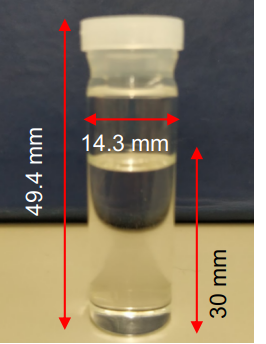
\includegraphics[width=4cm]{scintVial.png}
		\end{minipage}
	}
	\subfigure{
		\begin{minipage}[b]{0.35\textwidth}
			\centering
			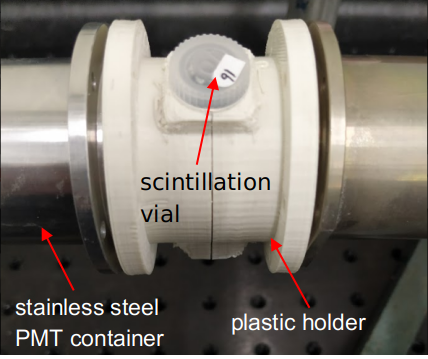
\includegraphics[width=6cm]{plasticHolder.png}
		\end{minipage}
	}
	\caption[A vial filled with the test sample and the measurement setup.]{A vial filled with the test sample (left) and the measurement setup (right). Left: The samples were filled into scintillation vials. The dimensions are shown in the picture. Right: two PMTs were aligned by a coupling to face the scintillation vial from each side.\label{scintVial}}
\end{figure}

Two Hamamatsu R580 PMTs (see Hamamatsu R580 manual\cite{pmtR580} for details) were used for detecting the light. The diameter of the PMT round surface is 38.71 mm. These PMTs were housed in stainless steel cylinders (PMT holders), set face to face, looking at the scintillation vial from each side. The PMTs and the vial were aligned by a plastic coupling, as shown in the right picture in Fig.~\ref{scintVial}. The plastic coupling is cylindrical, with a hole on the top into which the scintillation vial is seated, and a slot at the bottom to attach a radioactive source. Inside the cylindrical coupling there is a button-shaped groove at the bottom, to secure vial upright. At the bottom of the coupling, the center of the groove from inside is aligned with the center of the slot from outside. A 2-mm-diameter hole was drilled through the bottom center to allow the radiation rays to pass through the vial from the bottom. The surface inside the coupling was polished to be smooth to reduce its absorptivity. The coupling piece is made of plant-based and biodegradable polylactide (PLA) filament, and was machined by a 3D printing facility at U. Alberta\footnote{Shengzhao Yu, who was the undergraduate student at the Department of Physics, helped with the machining.}.

\begin{figure}[htbp]
	\centering	
	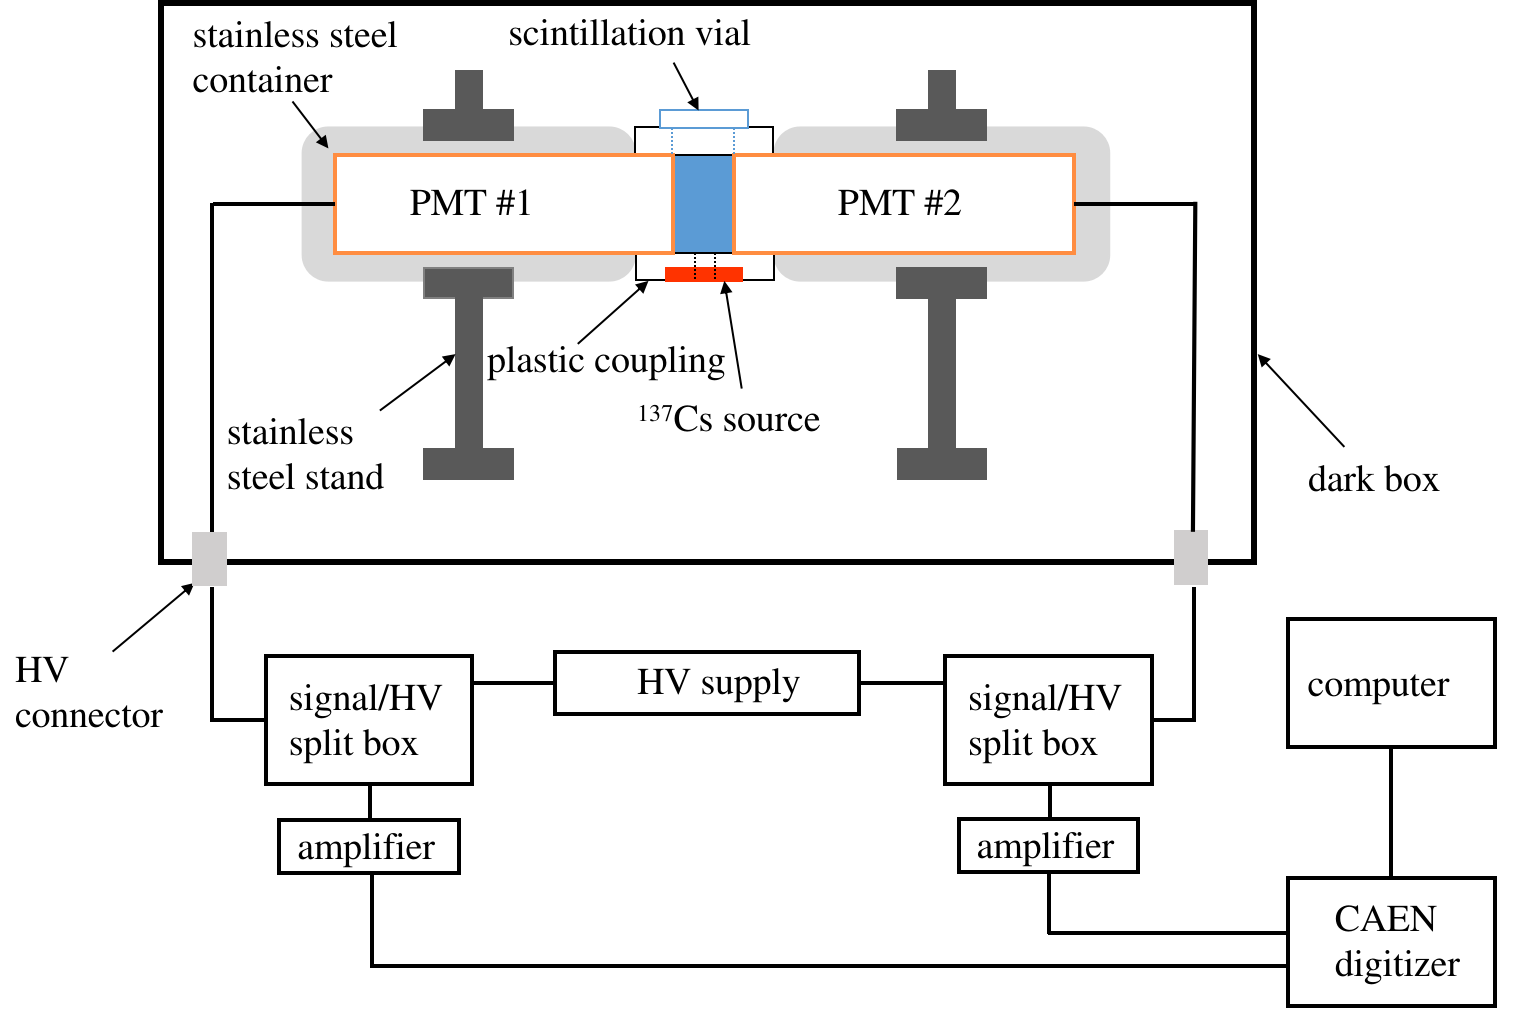
\includegraphics[width=10cm]{teLSsetup.png}
	\caption[A diagram shows the light yield measurement setup.]{A diagram shows the light yield measurement setup. See the text for details.}
	\label{teLSsetup}
\end{figure}

Fig.~\ref{teLSsetup} shows a diagram of the whole measurement setup. The plastic coupling piece held the radioactive source and the scintillation vial. It also aligned two PMTs to face the scintillation vial from each side, and shielded the vial from outside light. The apparatus was placed in a dark box to prevent light from the lab. Two RG59/U-type high voltage (HV) cables connected the PMTs to an HV supply outside the dark box. The HV cables were connected to two signal/HV split boxes to separate the HV current and electrical signals. Due to the resistance of the split box, the HV supply was set to 2200 Volts (V) for PMT operation, instead of the 1800 V operation voltage suggested by Ref.~\cite{pmtR580}. 

The signal cables from the split box were connected to a two-channel Hewlett Packard (HP) amplifier, which inverted the signals and amplified them by 26 dB. The amplified signals were then input to a two-channel digitizer whence they were recorded on a desktop computer.

To obtain and analyze the data, we used a desktop Waveform Digitizer, the DT5751 module provided by the Costruzioni Apparecchiature Elettroniche Nucleari (CAEN). Running in a digital pulse processing mode, the module records the digitized PMT waveforms with a data-taking rate of 1 GHz for each channel \cite{caen}.

This module was controlled by the \texttt{CoMPASS} software provided by CAEN. The software set up the threshold and trigger parameters. Once the triggered event passed the threshold, the software recorded event time, trigger flag, and waveform histograms from the two channels. By integrating the waveforms, the energy of a triggered event was calculated \cite{compass}.

Each channel recorded the signals from each PMT individually. With the two-PMT setup, we applied coincidence time mode measurements. In the coincidence mode, a coincidence time window between two channels was set to 48 ns. For a certain event, the \texttt{CoMPASS} software compares the event time difference between two channels and only records it if the event time difference is less than 48 ns. A smaller window of 10 ns was further applied for analysis.

\subsubsection{Measurement}

The liquid scintillator samples we have measured are LAB-PPO, TeDDA, and TeSOP. The unloaded LAB-PPO sample served as a standard candle.

A Cesium-137 ($^{137}$Cs) radioactive source was always placed at the bottom of the scintillation vials.
The source was made by Radiochemical Centre Amersham. The radioactivity measured on 1st April 1974 was $11.09 \, \mathrm{microcurie}(\mu\mathrm{Ci})$ on record, with an accuracy of $3.7\%$. Then the activity was expected to be 
$11.09\times ({\frac{1}{2}})^{\frac{46}{30.08}}=3.84 \, \mu\mathrm{Ci}$ in 2020, accounting for the 30.08 year half-life of $^{137}$Cs \cite{nndc}.

Upon decay, the $^{137}$Cs isotope has an 85.10\% chance to emit 0.661 MeV $\gamma$-particles \cite{nndc}. These $\gamma$-particles can travel into the liquid scintillator sample in the vial, interact with the samples, and create scintillation photons.

For each sample, measurements were taken for a one-minute time duration. Waveforms from the PMT photo-current signals were digitized in a 252 ns time window. Shown in Fig.~\ref{teLSwaveform} is a typical waveform caused by $\gamma$-particles interacting with the LAB-PPO sample. The photo-electron (p.e.) signals triggered PMT pulses, and the pulses were digitized as waveforms. For each waveform, the digitizer firmware dynamically calculated the baseline as the mean value of 256 data points inside a moving time window of 252 ns width. A threshold was set as 100 LSB (Least-significant bit) units above the baseline. The data point at 90\% of peak height on the leading edge of the pulse was taken as the trigger time ($trig$) tag.

After the occurrence of this $trig$ tag so as to avoid introducing another pulse, in the subsequent 80 ns window the digitizer did not produce another trigger (trigger hold-off). Also, from the $trig$ tag, a pre-gate of 8 ns was set. The waveform was integrated across the time interval $[trig-8, trig+72]$ ns. This gives the integrated charge, which was provided (i.e. output) in one of the A/D convertor's (output) channels. 

If the measurement system were to be calibrated, the ADC channel number could be converted exactly into the energy of the particle interaction. However since here we are interested only in the photon count, we used the ADC channel as the energy without further scaling. Once the pulse in the waveform passed the threshold and a triggered time tag was found, the digitizer considered it as a triggered event. A time flow started when the measurement began. Timestamps were recorded as event time when the triggered event happened. The waveform was recorded, and the ADC channel number (nominally, the energy) of this event was calculated.

\begin{figure}[htbp]
	\centering	
	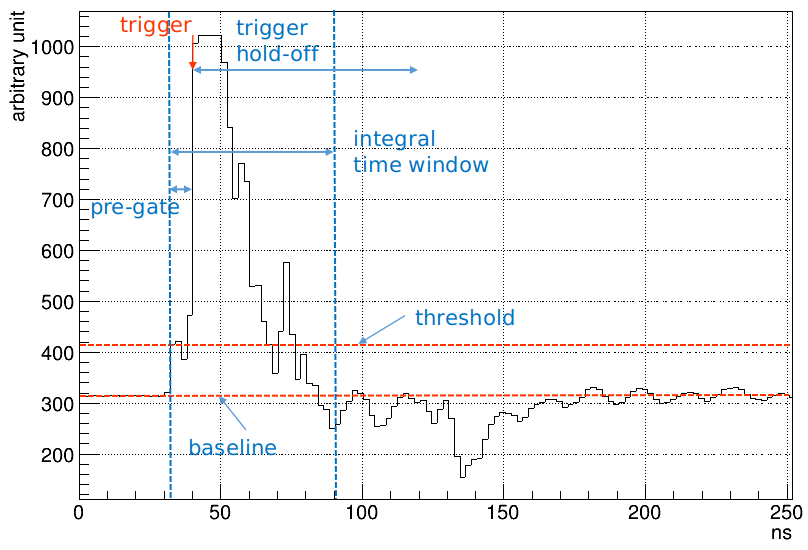
\includegraphics[width=8cm]{teLS_waveform.png}
	\caption[A typical triggered waveform.]{A typical waveform triggered by scintillation photons from $^{137}$Cs $\gamma$-particles interacting with LAB-PPO in the scintillation vial.}
	\label{teLSwaveform}
\end{figure}

In a coincidence time measurement, the event times of the events recorded by each of the two PMTs were compared. If the event time differences between two events from each PMTs were too long, those events were considered to be random noise rather than the physics events, and were not recorded. We optimized a coincidence time cut as 40 ns and set that cut during the digitizer data-taking. 

\begin{figure}[htbp]
	\centering	
	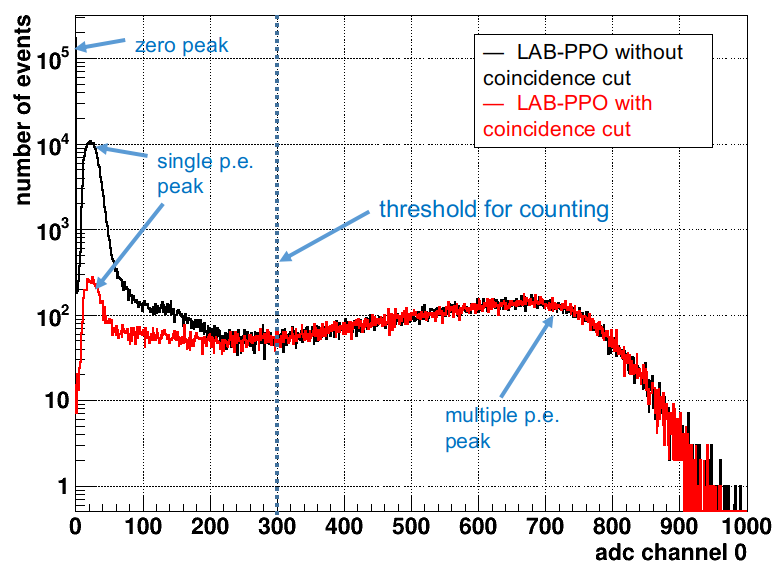
\includegraphics[width=10cm]{TeLScoinCut.png}
	\caption[Measured LAB-PPO energy spectrum with and without coincidence cut]{Measured LAB-PPO energy spectrum with and without a coincidence cut on the ADC channel 0. A threshold for counting is set by comparing the two spectra.}
	\label{teLScoinCut}
\end{figure}

Fig.~\ref{teLScoinCut} shows the measured LAB-PPO energy spectrum with and without coincidence time cut ($10$ ns) on a single ADC channel (here using channel 0). Without the coincidence time cut, there is a zero peak caused by the pulses from random electronic noise or fluctuations of the digitized waveforms. The peak on the left is the single p.e. peak. It is mainly caused by light sources (events) that are so weak that the captured photons produce at most one single photo-electron inside the PMT \cite{leo2012techniques}. The peak on the right is the multiple p.e. peak, in our case, which is mainly caused by scintillation photons produced by the ($^{137}$Cs) 0.661 MeV $\gamma$-ray interacting with the LAB-PPO. In the coincidence time measurement mode, the sampling system only records photons detected by the two PMTs almost simultaneously. Therefore, the zero peaks are removed and the single p.e. peak is suppressed. The multiple p.e. peak is consistent with the non-coincidence measurement. A threshold in energy, shown on Fig.~\ref{teLScoinCut} as 300 (nominal energy units) can be set to count only the scintillation photons emitted from LAB-PPO. 

\begin{figure}[htbp]
	\centering	
	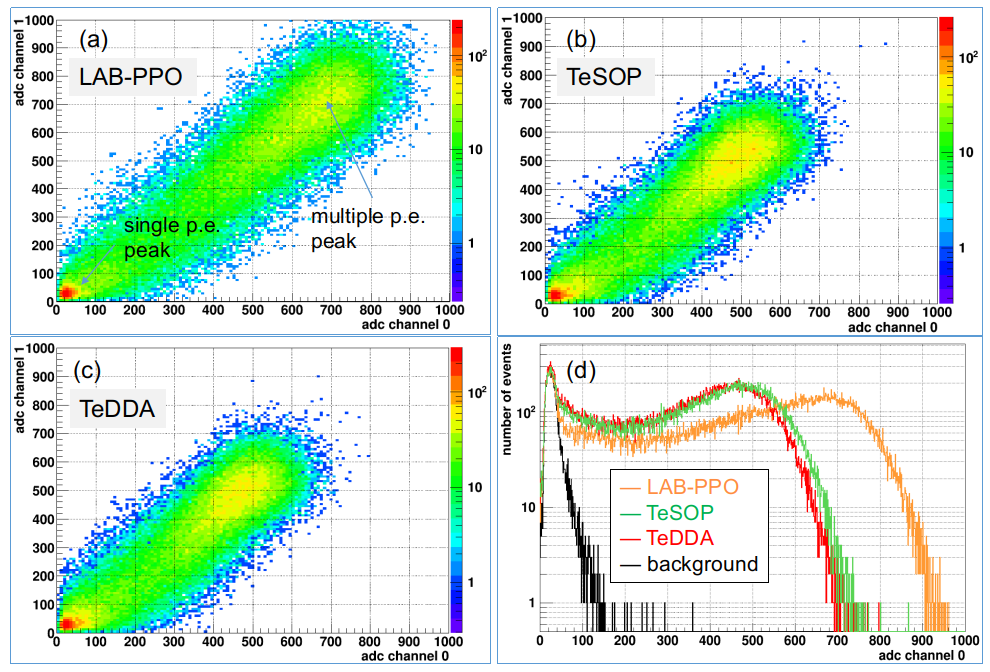
\includegraphics[width=14cm]{TeLS_2Denergy.png}
	\caption[The 2D energy spectrum of the counting measurements.]{The 2D energy spectrum of the counting measurements of LAB-PPO (a), TeSOP (b), and TeDDA (c) samples, projected the 2D plots into one channel (d). The single photo-electron (p.e.) peak is mainly caused by backgrounds while the multiple p.e. peak is from scintillation photons.}
	\label{teLSresults}
\end{figure}

Fig.~\ref{teLSresults} (a) shows the result of a one-minute measurement for the LAB-PPO sample. The data points in the 2D plot represent the triggered events read by the ADC channel 0 and 1 simultaneously. A 10 ns coincidence window cut was applied to cut down noise, single p.e., and background events. The events in the 0 ADC channel, which represent noises, were totally cut off after applying the coincidence cut. Fig.~\ref{teLSresults} (b) and (c) show corresponding results for the TeSOP and TeDDA samples respectively. Compared to the LAB-PPO sample, a shift of the multiple p.e. peak due to the different light yields can be observed clearly. %% John: confusions here

The 2D plots were projected onto a single channel, as shown in Fig.~\ref{teLSresults} (d). We used an empty vial and let $\gamma$-particles from the $^{137}$Cs source pass through it as a background run (without imposing the coincidence cut). This was to verify the single p.e. peak and noise region, shown as the black background spectrum. From this plot, the single p.e. peaks for all the samples and the background match together. The several different multiple p.e. peaks indicate the different light yields of the scintillator samples. Here we can see the multiple p.e. peak of the LAB-PPO occupies the largest ADC channel number, while the channels of TeSOP are slightly larger than the TeDDA. 

%\color{red}There are too many short paragraphs in the remainder of this section, Jie. I'm unable to make sense of it actually, and just had to give up. Sorry, I know writing in a language other than one's mother tongue is very challenging!\color{black}

To quantify the light yield differences between different samples, an analysis method of charge weighted photon number has been applied as the following:

First, from the energy spectrum, the single p.e. peak was fitted with an asymmetric Gaussian function ($f_{asym}$ in \ref{eq:asyGaus}), as shown in Fig.~\ref{fitSinglePE}. The mean value of the asymmetric Gaussian ($p_0$) represents the ADC channel number corresponding to the single p.e. peak for the weighting. 

\begin{equation}\label{eq:asyGaus}
f_{asym}=c \; \exp\left[- \frac{(x-\mu)^2}{2 \sigma^2} \, \right] \; \mathrm{Erfc}(\xi),
\end{equation}
where $\xi=-\frac{\alpha(x-\mu)}{\sqrt 2\sigma}$.

Then in the multiple p.e. region, weighting (dividing) the counts of the event in each channel with the single p.e. ADC channel number to calculate the total number of the photons.

\begin{figure}[htbp]
	\centering	
	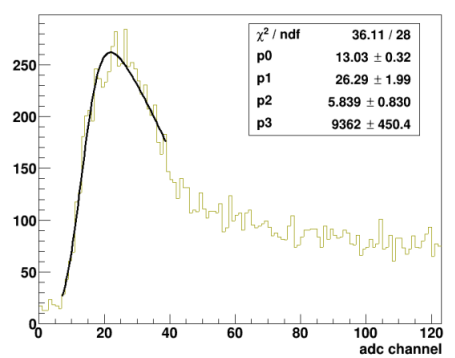
\includegraphics[width=6cm]{fitSinglePE.png}
	\caption[The single p.e. peak fitted with an asymmetric Gaussian function.]{The single p.e. peak is fitted with an asymmetric Gaussian function ($f_{asym}$) to obtain the ADC channel for weighting. The mean value of $p_0$ is used as the adc channel relative to a single p.e. peak.}
	\label{fitSinglePE}
\end{figure}

To define the multiple p.e. region for the counting, the spectrum projected on each channel with and without coincidence cut are compared to define a threshold of the ADC channel for counting. By integrating from this threshold, the total numbers of events between two spectrum are close to each other. From two channels, we get two thresholds and then define a box cut in the 2D coincidence plot. We weights the events in the box to obtain the total number of photons.
\begin{figure}[htbp]
	\centering	
	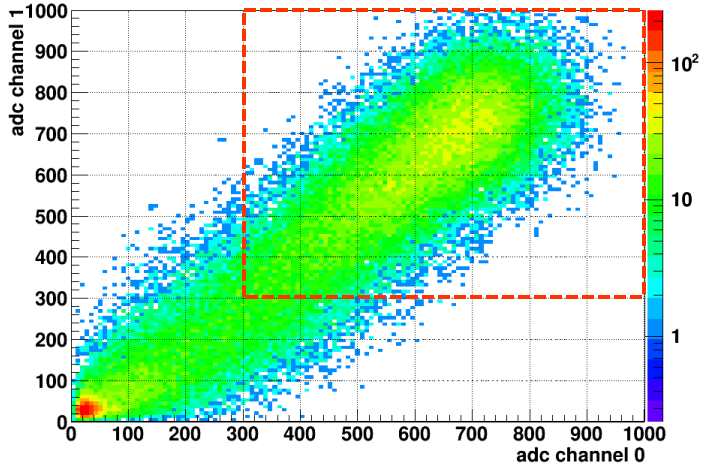
\includegraphics[width=6cm]{TeLS_2DboxCut.png}
	\caption[Two dimensional spectrum of LAB-PPO sample with coincidence cut.]{Two dimensional spectrum of LAB-PPO sample with coincidence cut. A box cut is defined for multiple PE counting.}
	\label{2DboxCut}
\end{figure}

Two dimensional (2D) spectrum of LAB-PPO with coincidence cut is shown in Fig.~\ref{2DboxCut}. A box cut is defined for multiple PE counting. 

Once the total number of photons for a certain sample is counted, we can calculate its ratio to the LAB-PPO sample to obtain the relative light yield.

\subsubsection{Results}
\begin{table}[ht]
	\centering
	\caption{\label{lightyield1} Number of photons calculated by Charge weighted photon number method.}
	\centering	
	\begin{tabular*}{100mm}{c@{\extracolsep{\fill}}cccc}
		\toprule 
		Sample & Number of photons ($\times 10^6$) & RLY\\
		\midrule
		LAB-PPO& 2.0811 & 1\\
		TeDDA& 1.2652 & 	0.61 \\
		TeSOP& 1.3976 & 0.67\\
		\bottomrule	
	\end{tabular*}
\end{table}

Table.~\ref{lightyield1} shows the number of photons calculated by the charge weighted photon number method. Here we quantify the relative light yields of our samples. The light yield of the $0.5\%$ Te by SOP synthesis procedure (TeSOP) is $0.67$ and the one of the $0.5\%$ Te by DDA procedure is 0.61. The light yield of TeSOP is slightly larger than the TeDDA. These results are close to the relative light yield of $\sim 0.65$ for the $0.5\%$ Te loading samples reported by Ref.~\cite{biller2017new}.

\section{SNO+ Electronics}

In this section, the SNO+ electronics system is introduced. The system includes the trigger and readout systems. As mentioned in \ref{sect:overview}, the PMTs as photon sensors are the basic detection elements for the SNO+ detector. The signals from the PMTs are sent to the SNO+ electronics system, which records the PMT time and charge information and then transfers the digitized data to offsite computing systems for data analysis. These steps are detailed in the following.

The photons created from particle interactions in the detector propagate to the PMT sphere and may hit a certain PMT and strike on its photo-cathode, which is a thin cesium bialkali film coated on the inner surface of PMT glass. The photocathode then produces a photo-electron (p.e.) through a photoelectric effect. The photocathode is held at ground voltage, while the anode is at a high voltage ranging from $+1700$ to $+2100$~V \cite{boger2000sudbury,dunger2018topological}. This potential difference establishes strong electric fields inside the PMT. The p.e. is accelerated and focused by the electric field in the PMT and travels through a volume which is under vacuum until it reaches the region of a series of secondary emission electrodes, called dynodes. When the p.e. transfers its energy to the material in the dynodes, a number of secondary electrons escape and form a measurable current, which is collected by a custom-made operating circuit (called ``PMT base'') at the anode \cite{hamamatsu2018photomultiplier}.

The anode pulse produced from the PMT travels along 35 m long RG59/U type coaxial cable (with a resistance of 75 $\Omega$) to the front-end electronics, which are located on the deck above the detector. The coaxial cable also carries the high-voltage \cite{boger2000sudbury}. 

To tidily manage the more than 9000 PMTs in the SNO+ detector, the coaxial cables connected to the PMTs are grouped into bundles. Each bundle is connected to a Paddle Card, which is linked to a PMT Interface Card (PMTIC). The PMTIC supplies the high voltages and receives the signals from the PMTs. 32 channels (for 32 PMTs) in the PMTIC are plugged into a Front End Card (FEC) that processes, digitizes, and stores those 32 PMT signals. There are in total over 300 of the Front End Cards, distributed (or organized) across 19 `crates' to energize and monitor the 9728 PMT channels in total. Of that total, 32 channels are reserved for calibration inputs and labeled as FEC Diagnostic (FECD) channels. These FECD channels are mainly used to tag calibration events. The triggered PMTs can be labeled by the logical channel number (lcn) using the map of the PMT to the crates and cards \cite{snop_jinst,stringer2019sensitivity}:
\begin{equation}
\mathrm{lcn = 512 \times crate + 32 \times FEC + channel}.
\end{equation}

A 10-MHz and a 50-MHz clocks are used to record the time of the triggered event. The universal time of the triggered event is calculated as the time elapsed from a predefined origin $zero$, namely midnight on January 1, 2010 (GMT), until the moment when the event happens. A 10-MHz clock used for counting the absolute time started at $zero$. It has a 53 bit register and can run for 28.5 years. Its accuracy is maintained by a GPS system. The 50 MHz clock gives more accurate timing. It limits the best time resolution of the global trigger time (GT) to 20 ns. This clock has a 43 bit register and rolls over every 2.04 days. The relative time between the events can be used for analyzing specific physics processes, such as radioactive decays \cite{rattime,stringer2019sensitivity}. 

The recorded hit information of the triggered event, including the time and charge information of hit PMTs and the trigger settings, are sent to a Crate Controller Card (XL3) in each crate. These cards were installed for SNO+ to handle higher data transfer rates compared to SNO, with a maximum rate of 14 MB/s, which is sufficient for typical data-taking rates of $~2.5$ MB/s \cite{bonventre2014neutron,rumleskie2021sno+}. The XL3 cards read the recorded data, wrap them as ethernet packets, and send them to the Data Acquisition System (DAQ) and Event Builder system \cite{walker2016study}. The Event Builder system writes information into event records based on their GT identification number (GTID) and saves them on storage disk \cite{snop_jinst}. These raw data are written to the disc and are further processed into ROOT format by high-performance computing clusters.

The SNO+ electronic system can measure signals with a nanosecond-level timing resolution and a single-photon level charge resolution. It can handle a ``routine'' event rate of several kHz, and when called for can handle much higher rates for cases such as the burst events from a galactic supernova \cite{snop_jinst}.

\section{Calibration}\label{sect:calibr}

Calibration sources with known physics parameters are operated frequently to determine the detector's response to well understood events, and essential step for making accurate measurements. Two kinds of calibration sources are used by SNO+: (1) optical sources to measure the \emph{in-situ} optical properties of the detector medium and to calibrate the PMT responses \cite{snop_jinst,anderson2021optical}; and (2) radioactive sources to test the detector energy response, check the performance of event reconstruction algorithms for reconstructing event position, direction and energy, and determine the systematic uncertainties in event reconstruction. The various radioactive sources designed for SNO+ cover the energy range from 0.1 MeV to about 10 MeV, as listed in Table.~\ref{tab:radioSource} \cite{snop_jinst}. All the calibration sources have been designed to meet the radiopurity required by SNO+, and their materials are compatible with the detection media \cite{snop_jinst}.

\begin{table}[ht]
	\centering
	\caption[A list of SNO+ radioactive sources.]{A list of SNO+ radioactive sources for detector calibration. The energy cited is given the total $\gamma$ energy, modified from Ref.~\cite{snop_jinst}.}
	\label{tab:radioSource}
	\begin{tabular*}{60mm}{c@{\extracolsep{\fill}}cc}
		\toprule
		source & total $\gamma$ energy [MeV]\\
		\midrule
		\vspace{1mm}
		$^{16}$N  & 6.1\\
		AmBe & 4.4\\
		$^{46}$Sc & 2.0\\
		$^{48}$Sc & 3.3\\
		$^{137}$Cs & 0.66\\
		$^{57}$Co & 0.14\\		
		\bottomrule
	\end{tabular*}
\end{table}

Amongst these radioactive sources, the Nitrogen-16 ($^{16}$N) calibration source and the Americium Beryllium (AmBe) source have been deployed in the water phase and the partial-fill phase. The $^{16}$N source was used to test and optimize the reconstruction algorithm discussed in Chapter 4. It was also used to obtain the reconstruction uncertainties in the water phase, which is the topic of Chapter 5. A detailed description of $^{16}$N source is given in Sect.~\ref{sect:n16}. 

The $^{46}$Sc, $^{48}$Sc, $^{137}$Cs and $^{57}$Co sources are newly designed by SNO+ to calibrate the energy scale in the scintillator and tellurium-loading phases, especially for the energy region of interest (ROI) in the $0\nu\beta\beta$ study \cite{snop_jinst}. 

The detector geometry is not perfectly symmetric due to the presence of the AV neck, ropes, gaps between the PMTs, and the differences between individual PMTs \cite{snop_jinst}. The deployment of calibration sources at different positions in the detector can help to understand the asymmetries in the detector response. To achieve this, several fixed optical sources were mounted at different positions on the PSUP. To provide a wider range in calibration source positions a source manipulator system (SMS) was installed, as shown in Fig.~\ref{fig:sms}. Sources are attached temporarily to (and removed from) the SMS via the Universal Interface (UI), which is a sealed, cylinder-shaped glove box on the top of the AV: this prevents Radon-bearing air in the lab from leaking into the detector. The motion of the deployed sources along the central vertical axis inside the AV is controlled by the Umbilical Retrieval Mechanism (URM) through an umbilical and a central rope, and the off-axis motion is controlled by the side rope manipulator system. The motion of the sources in the external water region between the AV and PSUP is along the calibration guide tubes \cite{snop_jinst}.

\begin{figure}[!htb]
	\centering
	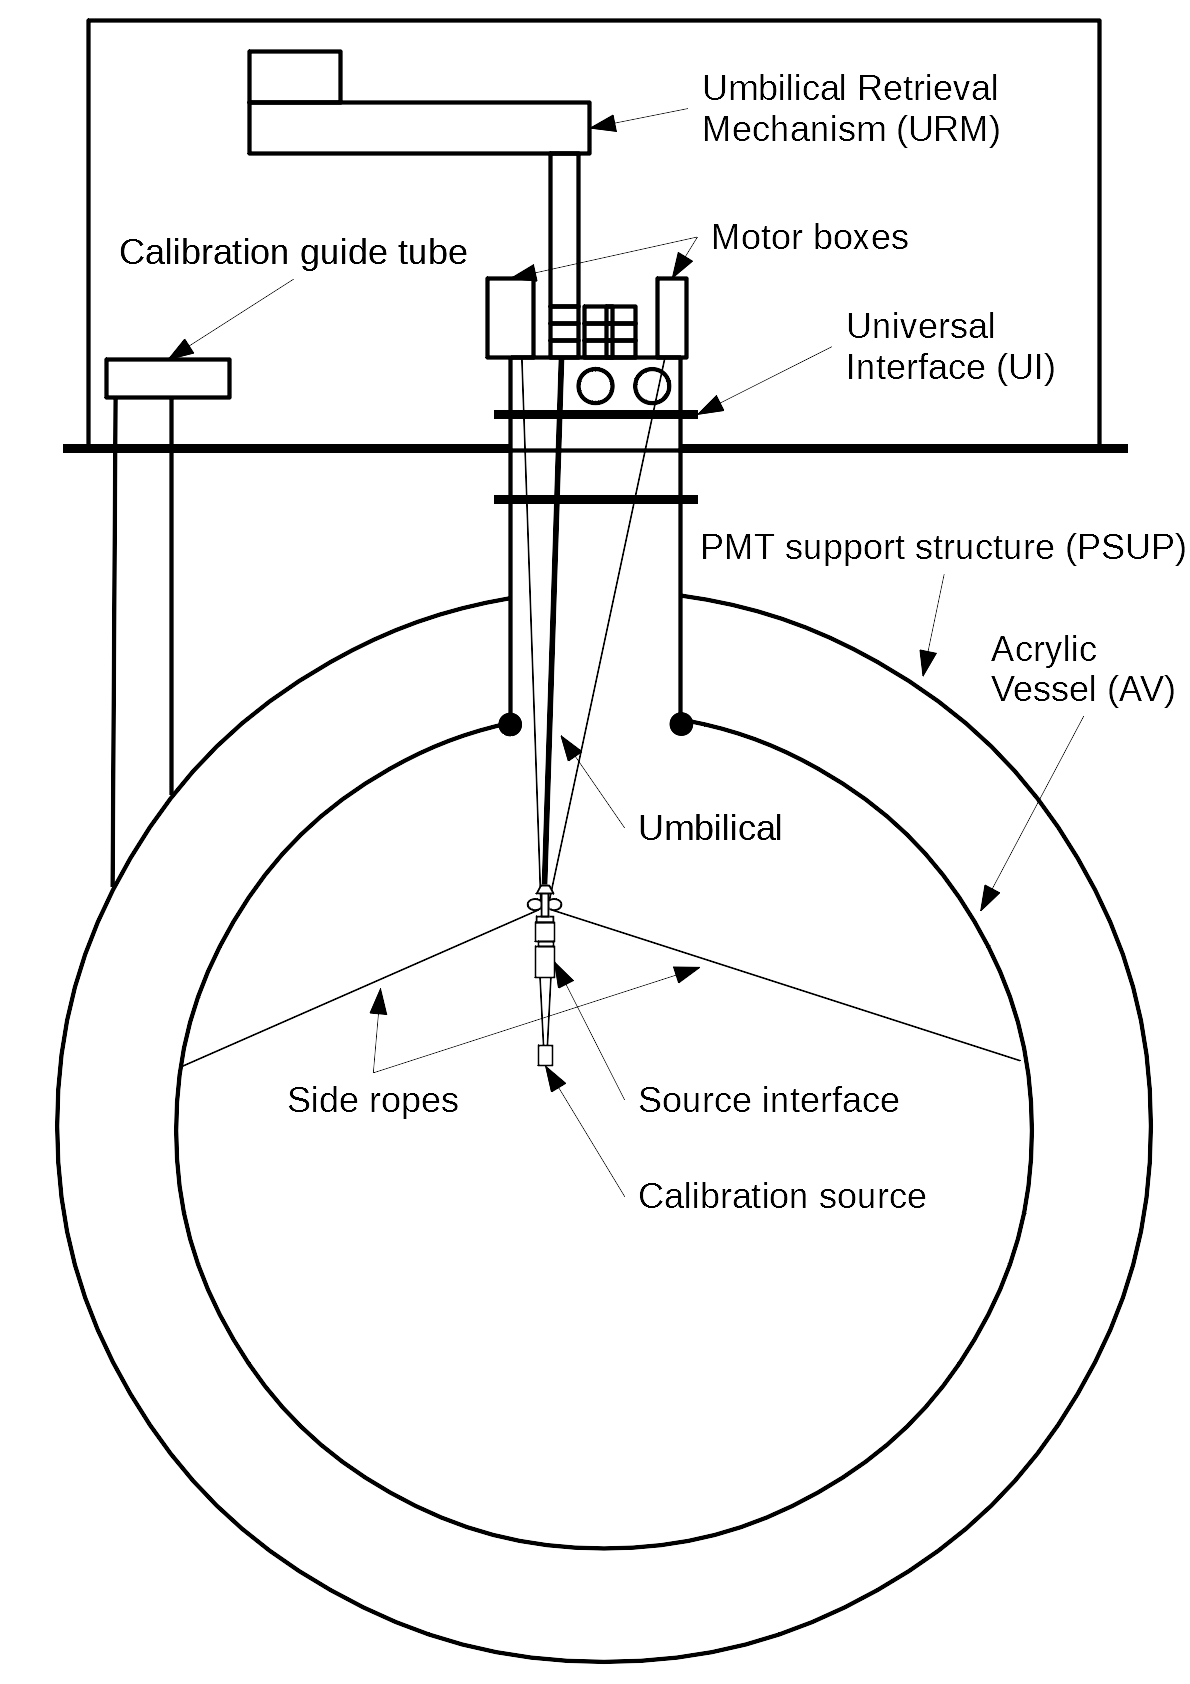
\includegraphics[width=8cm]{SMS.png}
	\caption[The SNO+ Source Manipulator System.]{The SNO+ Source Manipulator System, from Ref.~\cite{snop_jinst}.}
	\label{fig:sms}
\end{figure}

The position of the deployed source in the detector can be evaluated by the manipulator system. In addition, a camera system with six underwater cameras already mounted on the PSUP can take photographs of the source and then triangulate its position. A positional uncertainty of only a few centimeters is achieved. This system is also used to monitor the physical state of the detector, such as the offset of the AV center with respect to the PSUP, the movement of the rope net, the height of the water-scintillator interface during the partial-fill, etc \cite{singh2020underwater,snop_jinst}.

\subsection{The $^{16}$N Calibration Source}\label{sect:n16}

The $^{16}$N calibration source was inherited from the SNO experiment, and is well-understood \cite{dragowsky1999sudbury,dragowsky200216n,hamer2001energy}. Fig.~\ref{n16pic} shows the geometry of the $^{16}$N source chamber. The chamber is a stainless steel cylinder mainly containing a small PMT and a gas decay chamber. The chamber was designed to confine the electrons from $^{16}$N decay within the chamber and let them be detected by the PMT inside \cite{dragowsky1999sudbury}.

\begin{figure}[!htb]
	\centering
	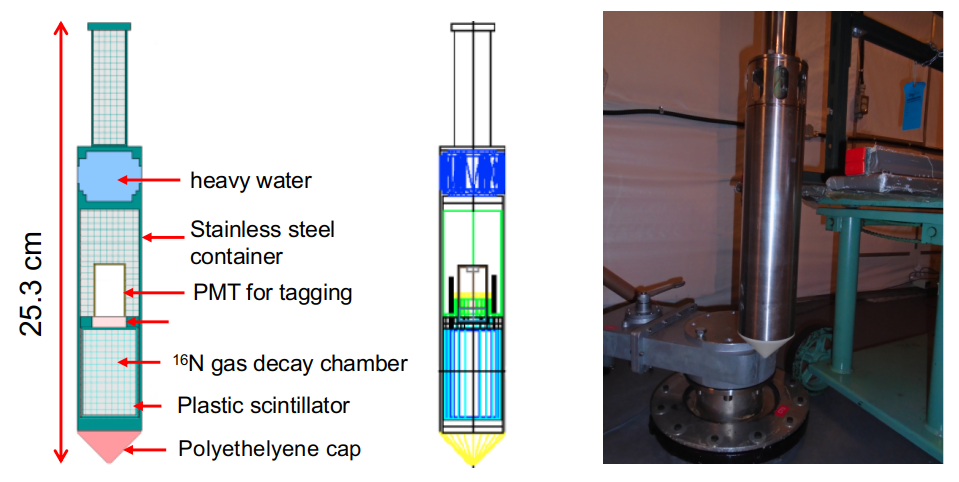
\includegraphics[width=12cm]{n16geom.png}
	\caption[$^{16}$N calibration source geometry.]{$^{16}$N calibration source geometry. Left: a detailed diagram of $^{16}$N source geometry, modified from Refs.~ \cite{maclellan2009energy,matt_deployedsource}; middle: source geometry implemented in RAT, modified from Ref.~\cite{n16geom_zach}; right: a picture of the $^{16}$N source, taken from Ref.~\cite{n16pic}.}
	\label{n16pic}
\end{figure}

Since the $^{16}$N isotope has a short half-life of $7.13$ s, it must be produced on-site during the calibration runs. A commercial deuterium-tritium (DT) generator was installed (underground) at SNOLAB to produce neutrons through the reaction: $D+T\to n \, + \, ^{4}$He; then the produced 14 MeV neutrons interact with CO$_2$ gas streaming through small diameter capillary tubing and produce the $^{16}$N isotope via the $(n,p)$ reaction: $n \, + \, ^{16}\mathrm{O} \to ^{16}\mathrm{N} \, + \,p$. These $^{16}$N nuclei are transferred into the cavity or detector via the CO$_2$ gas tubing \cite{dragowsky200216n}.

The $^{16}$N isotope mainly decays by $\beta$-decay process: $^{16}$N$\to ^{16}$O$+e^-+\bar{\nu}_e$. In doing so has a 66.2\% probability of emitting an electron with $E_{\mathrm{end~point}}=4.29$ MeV and a 22.8\% probability of emitting an electron with $E_{\mathrm{end~point}}=10.42$ MeV; furthermore the resulting $^{16}$O daughter nucleus de-excites, producing a cascade of $\gamma$-particles. These are mainly 6.13 MeV $\gamma$ particles with a probability of 67.0\% and 7.12 MeV $\gamma$ particles with a probability of 4.9\%. The probabilities of the $\gamma$-particles with other energies are all below 1\% \cite{nndc}. A simplified decay scheme is shown in Fig.~\ref{n16decay}.

\begin{figure}[!htb]
	\centering
	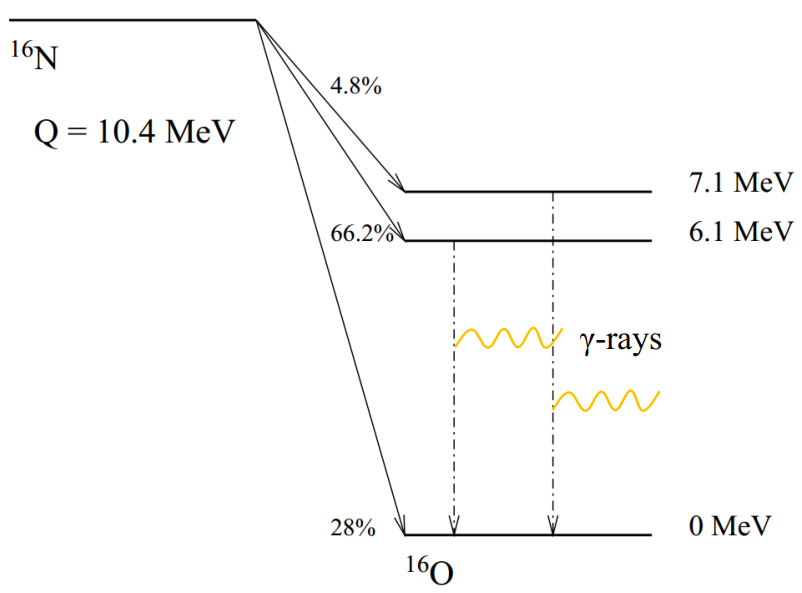
\includegraphics[width=6cm]{n16_decay.png}
	\caption[$^{16}$N main decay scheme]{$^{16}$N main decay scheme, modified from Ref.~\cite{dragowsky200216n}.}
	\label{n16decay}
\end{figure}

Calibrations using the $^{16}$N source are crucial for the quality of the reconstruction algorithms. Chapter 4 will cover how this source was used to test and optimize the reconstruction algorithms. Chapter 5 will show how the source is used to estimate the reconstruction uncertainties.

\section{Monte Carlo Simulation and RAT Software}\label{sect:rat}

The SNO+ collaboration uses a software package called the Reactor Analysis Tool (\texttt{RAT}) for Monte Carlo simulation as well as event-based analysis offline and online. To accomplish these two tasks, \texttt{RAT} integrates the \texttt{Geant4} simulation toolkit \cite{agostinelli2003geant4} and ROOT data analysis framework \cite{brunroot} for processing and analyzing data. This feature makes it easy to analyze Monte Carlo-generated events and real data in a same framework and data structure.

The software was originally developed by Stan Seibert from the Braidwood Collaboration to simulate a generic KamLAND-like detector \cite{ratManual}. A simulation package called Generic Liquid Scintillator \texttt{Geant4} simulation (\texttt{GLG4sim}) was developed and implemented in \texttt{RAT} \cite{horton2006introduction}. It simulates the scintillation physics, i.e. generation of scintillation photons and their propagation, reflections, refraction, scattering and absorption \cite{dunger2018topological}.

The SNO+ version of \texttt{RAT} links the existing \texttt{ROOT}, \texttt{Geant4} and \texttt{GLG4sim} packages to minimize code duplication. The SNO+ \texttt{RAT} is being developed by the whole collaboration and evolves with the experiment's progress to precisely simulate the SNO+ detector in its different physics phases, as well as being applied for many analysis tasks. The relatively flexible code structure of \texttt{RAT} allows the user to introduce their own code into the simulation or analysis process \cite{ratManual}. It can be updated and optimized with the measured parameters from detector calibration; it can be equipped with more precise descriptions of the physical processes in the detector; it can also be introduced with more advanced analysis tools. Users can perform different analysis tasks, such as using different reconstruction algorithms on the same set of events \cite{ratManual}. Therefore, different versions of \texttt{RAT} appropriate to and serving different SNO+ physics phases may give different outputs. For the work in this thesis, multiple \texttt{RAT} versions were used, mainly the versions for the water phase and the partial-fill phase. In this case, I will specify the \texttt{RAT} version when I discuss a specific analysis.

\texttt{RAT} is also used by other astroparticle physics experiments, such as the dark matter experiment DEAP/CLEAN \cite{caldwell2014simulation}. 
